%%%%%%%%%%%%%%%%%%%%%%%%%%%%%%%%%%
\subsection{APA Frame Mounting Structure and Module Securing}	
\label{sec:fdsp-pd-assy-frames}

\Dword{pd} modules are inserted into the \dword{apa} frames through ten slots (five on each side) and are supported inside the frame by stainless steel guide channels.  The slot dimensions for the \dword{spmod} \dword{apa} frames 
are \SI{136.0}{mm}$\times$\SI{25.0}{mm}\footnote{For \dword{pdsp} they were only \SI{108.0}{mm}$\times$\SI{19.2}{mm}; the increase allows for larger \dword{pd} modules and an increase in light collection area of nearly 50\% over the \dword{pdsp} design.}   
(see Figure~\ref{fig:pds-pd-mounting}~(left)).
The guide channels are positioned into the \dword{apa} frame prior to application of the wire mesh, and are not accessible following wire wrapping. Following insertion, the \dword{pd} modules are fixed in place using two stainless steel captive screws.

\begin{dunefigure}[\dshort{pd} mounting rails in \dshort{apa} frame]{fig:pds-pd-mounting}
{\dword{pd} mounting in \dword{apa} frame: Fixed end of PD module inside transparent APA side tube showing clearance for \dword{ce} cables (left) and showing \dword{pd} mounting rails in an APA frame  (right).}
	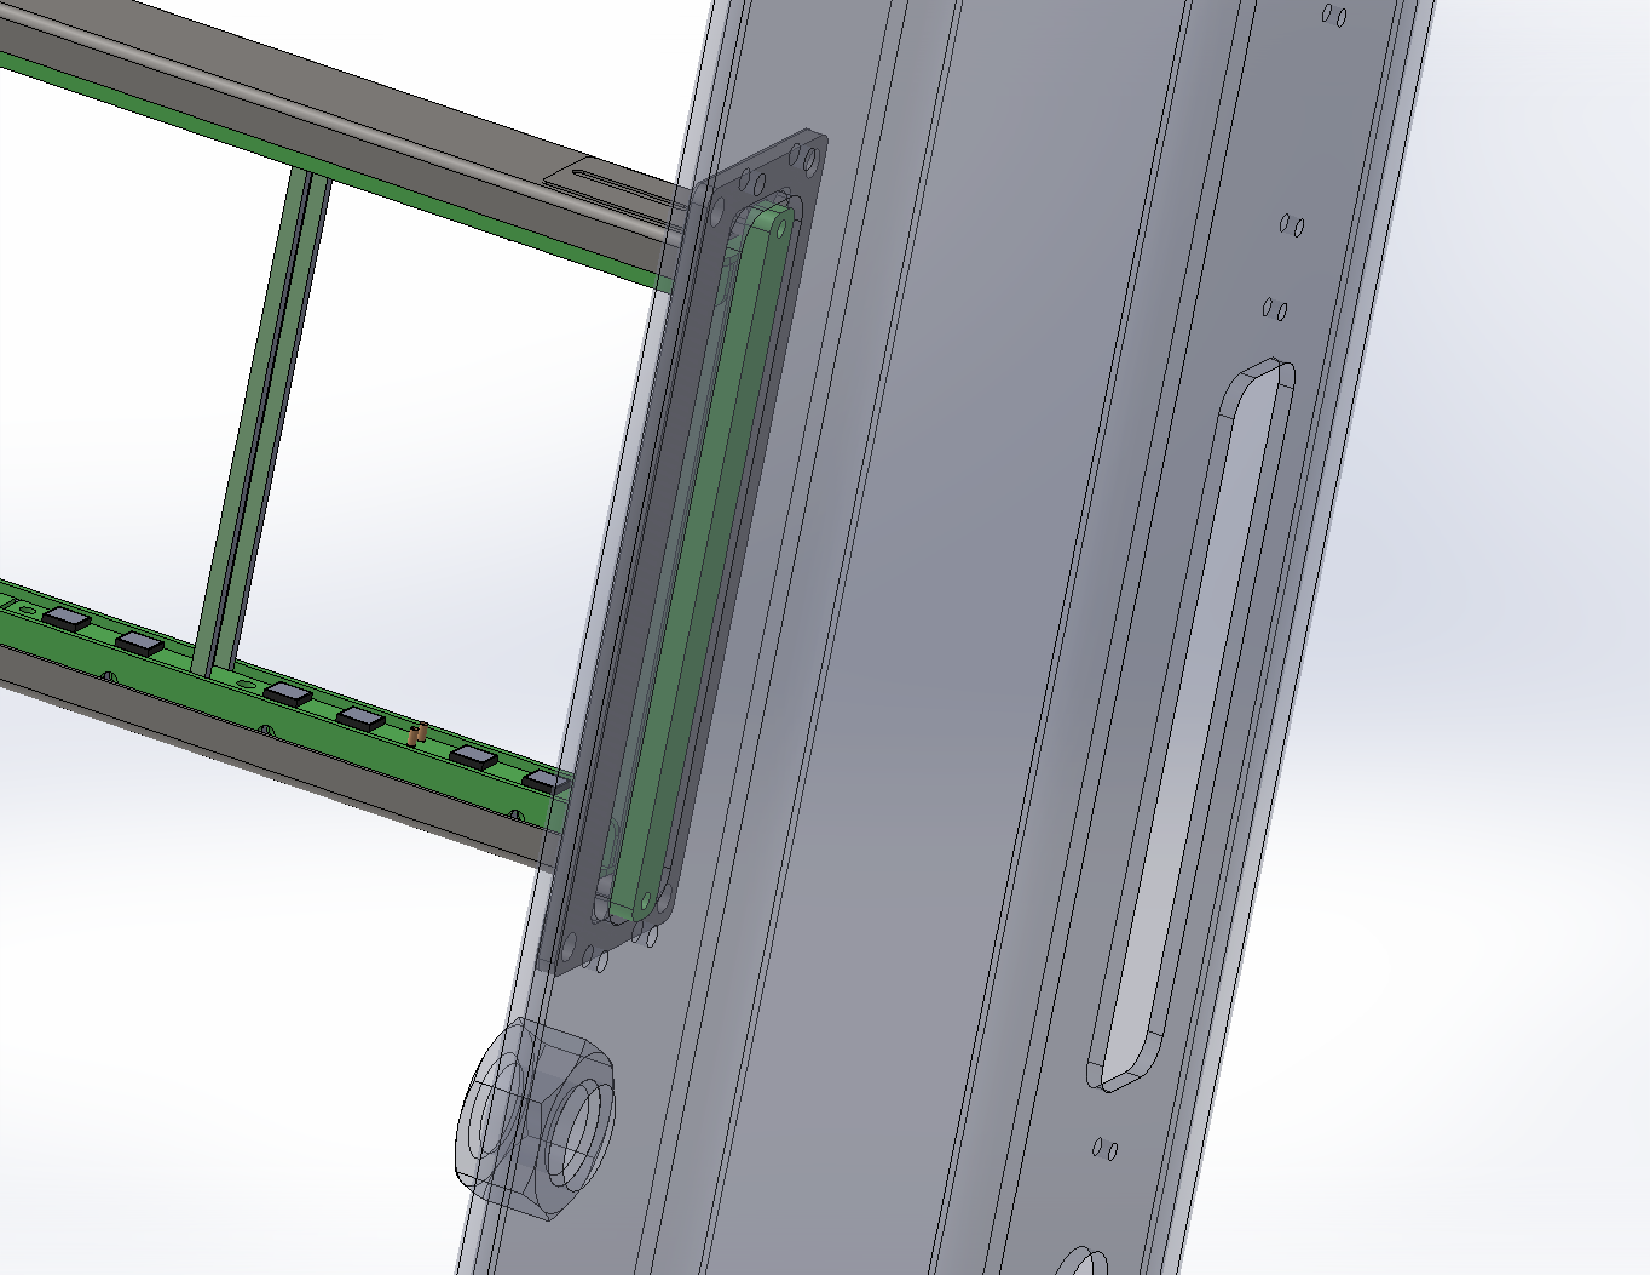
\includegraphics[height=6.cm]{pds-apa-pd-mounting-fixation}
	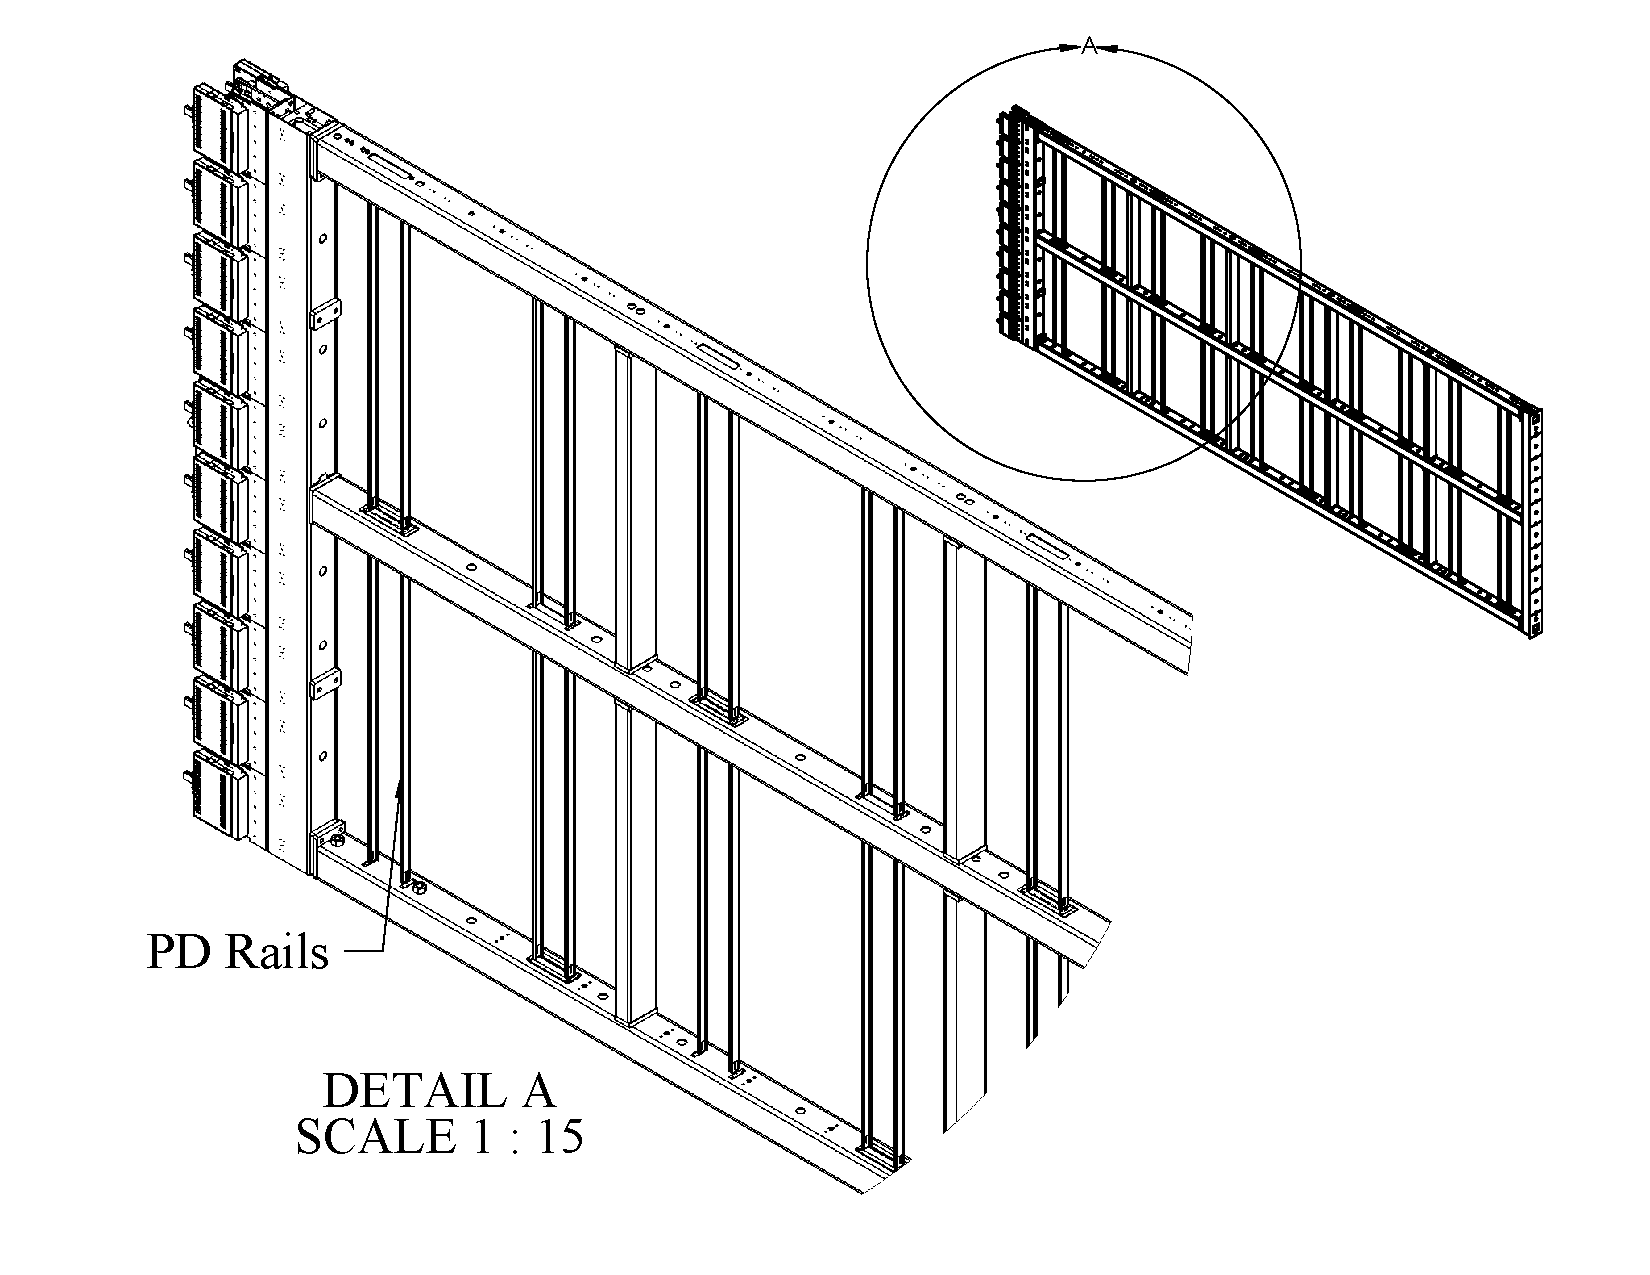
\includegraphics[height=6.cm]{pds-apa-pd-rails}
\end{dunefigure}

\subsubsection{Signal cable and connections}

For the \dword{pdsp}, \dword{pd} cables were run inside the \dword{apa} side tubes, five cables per side.  For the \dword{spmod}, however, this space will be filled by the cable harness for the lower \dword{apa} cold electronics (\dword{ce}) cables.  This change required a revised plan for placing the \dword{pd} cables.  In addition, it was observed during \dword{pdsp} \dword{pds} installation that running the \dword{pd} cables and making electrical connections to the modules during \dword{pd} integration was time-consuming and introduced risk to the process.

For the \dword{spmod}, the \dword{pd} cables will be %pre-
positioned in the \dword{apa} frames prior to installing the %ground shield 
mesh and wire-wrapping the frame.  
An \dword{apa} in the lower position will house the cables for only the \dwords{pd} in that lower \dword{apa} whereas those in the top position will house the cables for the upper \dword{apa} \dword{pd}s and the pass-through cables from the lower \dword{apa}. The cabling thus requires two different styles of \dword{apa} frame. All cables terminate at the header of the top \dword{apa} after assembly (see Figure~\ref{fig:pd-cable-routing-apa-frames}).

%\fixme{changed the description of the PD cable dww 10/11/19}

The cable connections between the upper and lower \dword{apa}s are made during \dword{apa} installation into the cryostat, while the \dword{apa} stack is being assembled. The same in-line multi-pin connectors used at the flange penetration in \dword{pdsp}\footnote{Hirose LF 10WBP-12S connectors https://www.hirose.com} are used for this connection.  Superior-Essex \footnote{http://superioressexcommunications.com} Category 6A U/FTP (STP) with FEP jacket (part no. 6S-220-xP) was validated in \dword{pdsp}.  Similar cable will be used in \dword{dune}, but custom-fabricated by the same vendor with two additional twisted pair contained within the external jacket for powering the photosensor active ganging board.

The \dword{pd} signal cables are expected to contract approximately 2\% relative to the \dword{apa} frame during cool-down of the \dword{detmodule} to cryogenic temperatures.  The design accounts for this by leaving cable loops in place between the anchor points to the \dword{apa} frame, allowing for the required relative motion.

To remove interference with the \dword{ce} cables, the electrical connections between the \dword{pd} modules and the \dword{pd} cable harness are moved to the face of the central \dword{apa} tube.  Printed circuit boards with spring-loaded electrical sockets are positioned on the inside face of the tube as part of the \dword{pd} rail installation as shown in Figure~\ref{fig:pd-cable-connectors}~(left).  During \dword{pd} integration into the \dword{apa} frames, a PCB with pin contacts mounted to the \dword{pd} module (see Figure~\ref{fig:mounting-board-routing-board}~right) engages into the PCB mounted to the \dword{apa} frame, automatically making the electrical connection as shown in 
Figure~\ref{fig:pd-cable-connectors}~(right).

\begin{dunefigure}[\dshort{pd} cable routing in \dshort{apa} frames]
{fig:pd-cable-routing-apa-frames}
{\dword{pd} cable routing in \dword{apa} frames: bottom \dword{apa} (left) and top \dword{apa} (right).}
	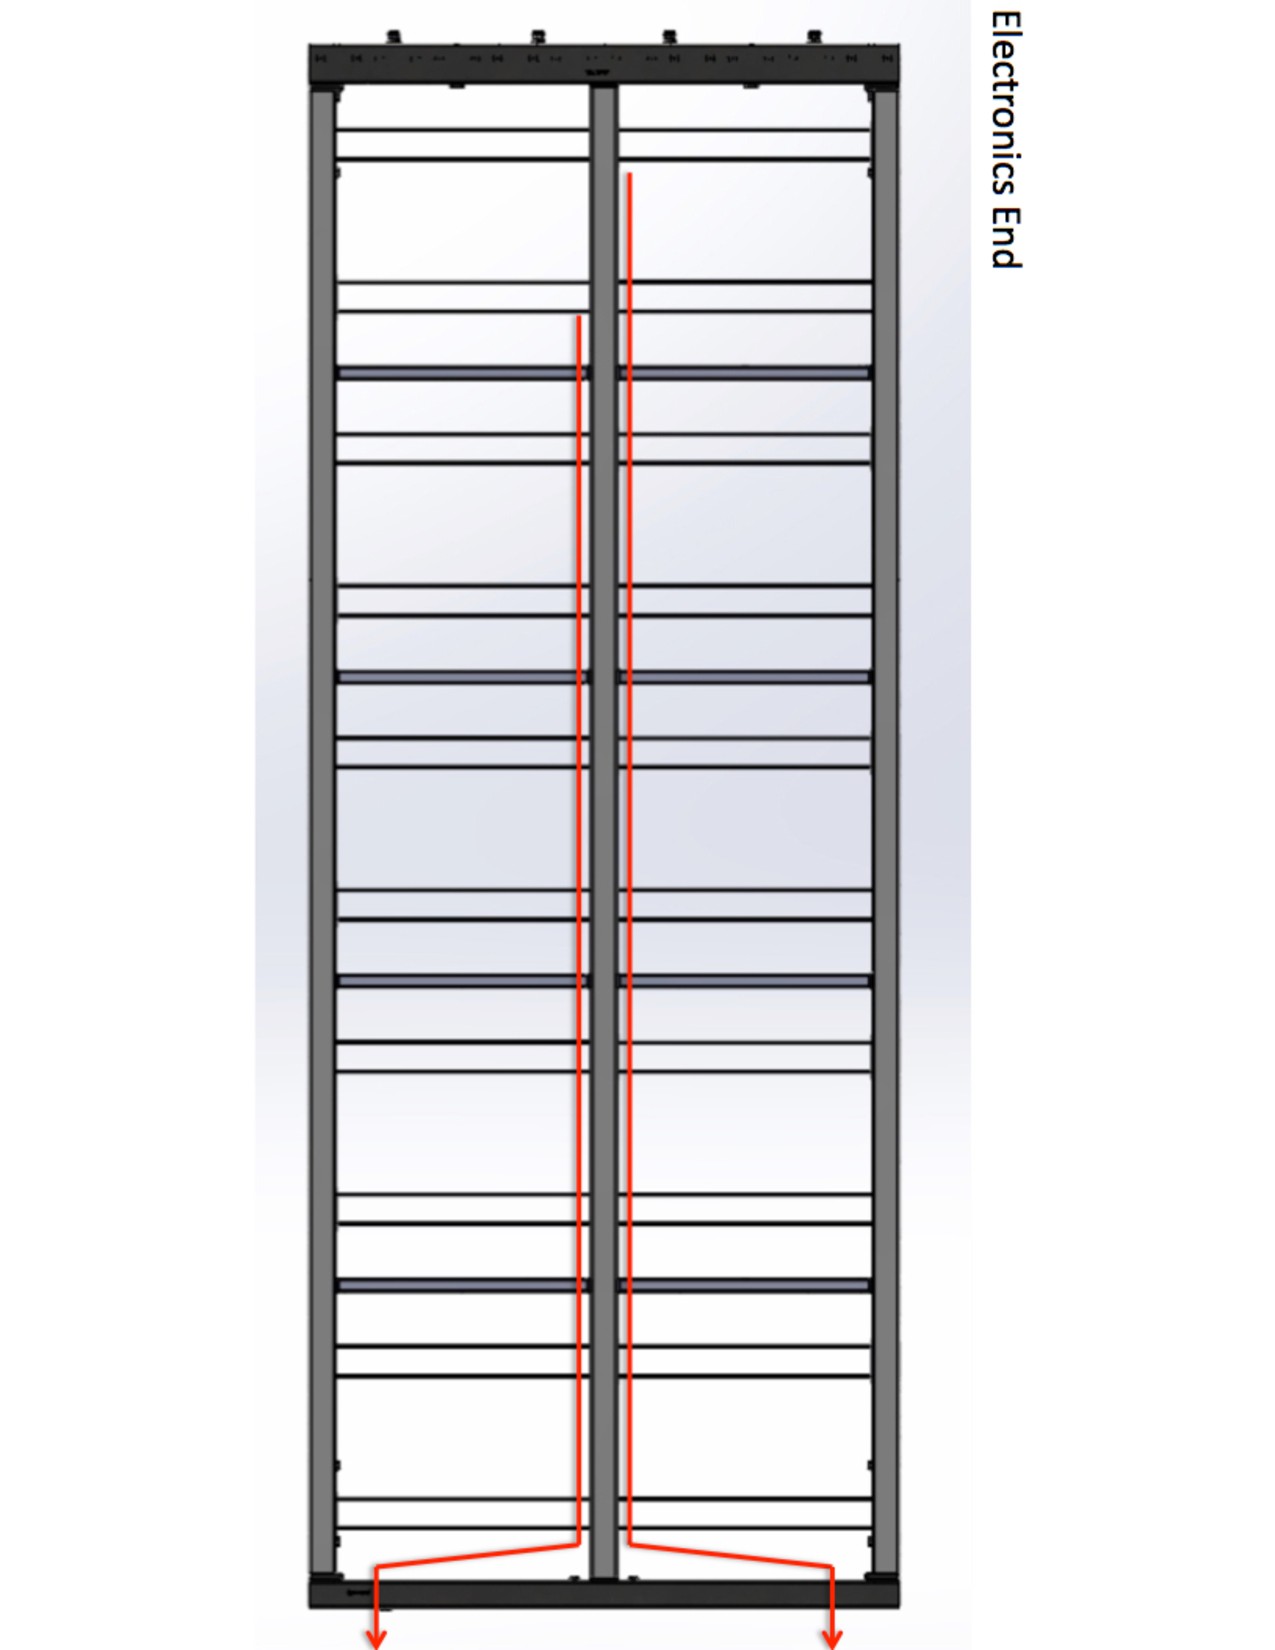
\includegraphics[angle=90,height=6.6cm]{pds-lower-apa-pds-cable-routing}
	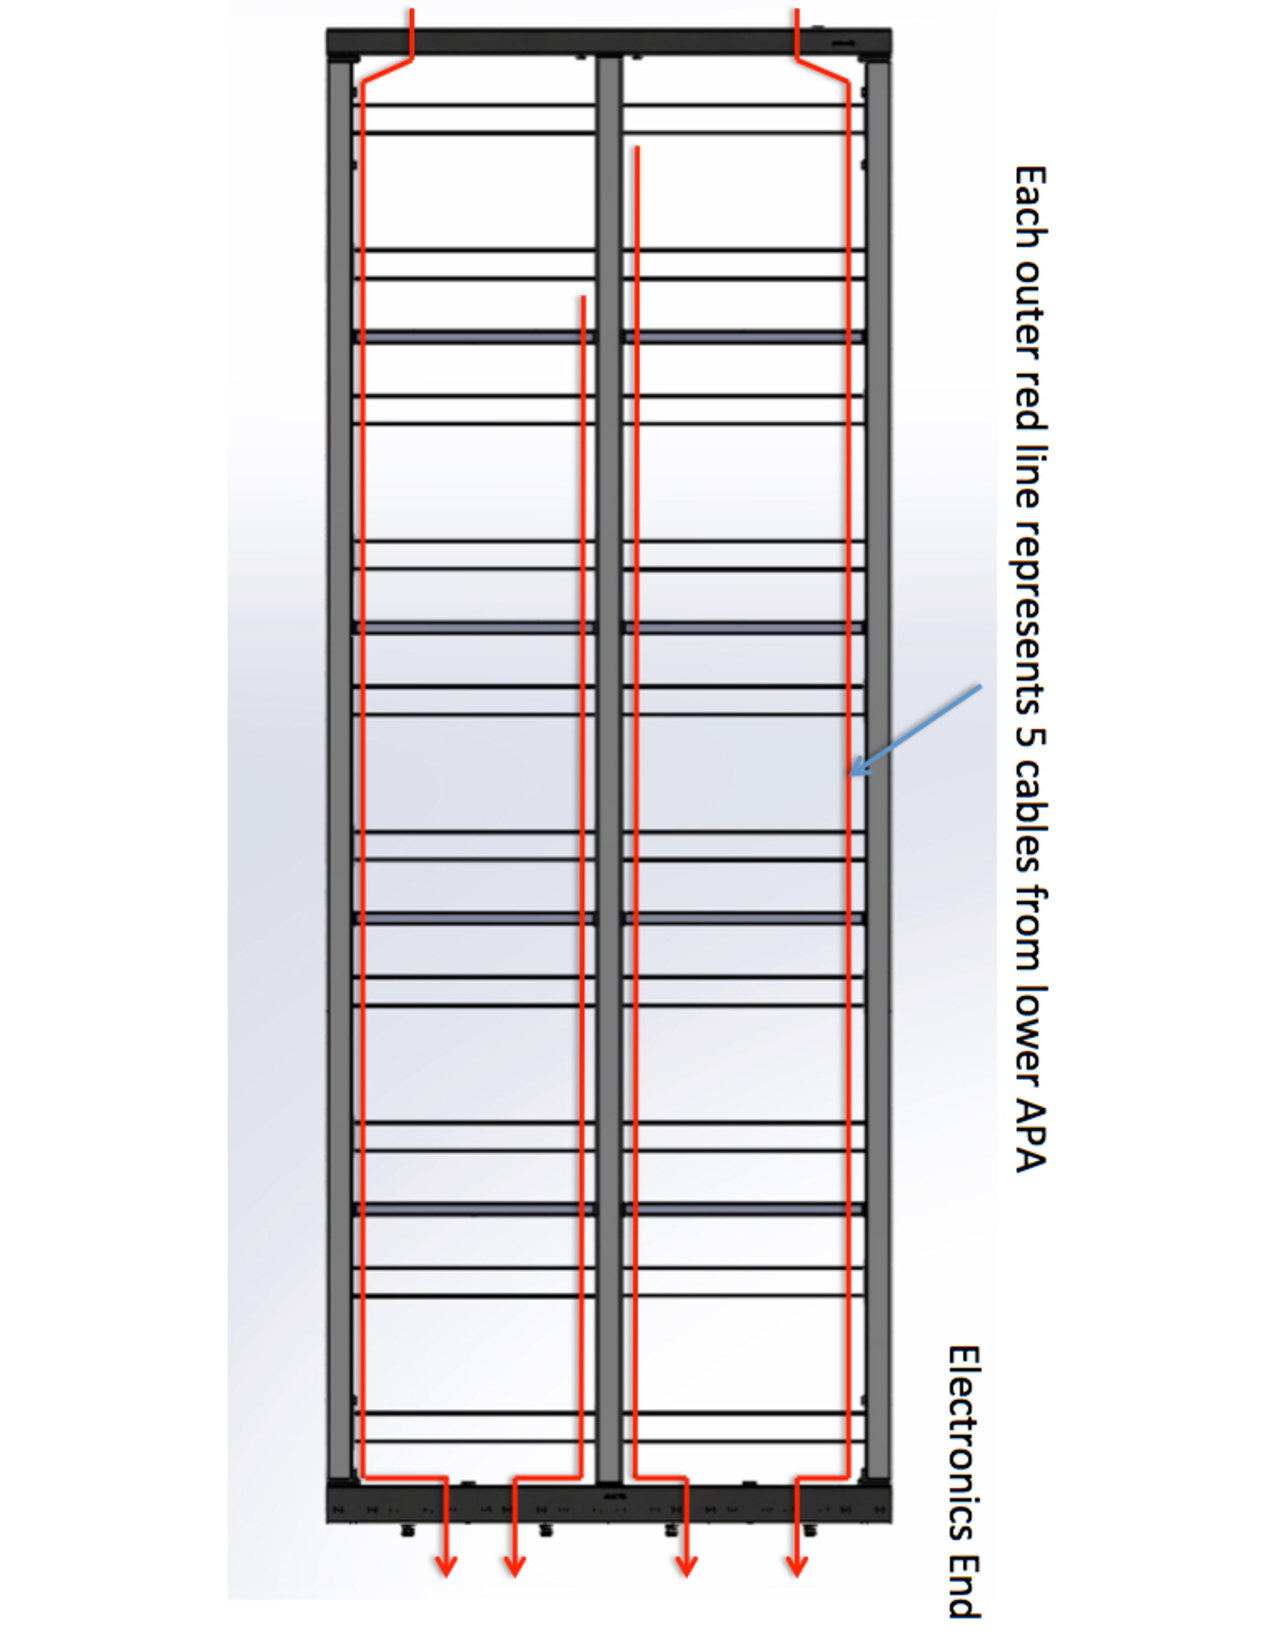
\includegraphics[angle=90,height=6.6cm]{pds-upper-apa-pds-cable-routing}
	\vspace{-1.5cm}
\end{dunefigure}

\begin{dunefigure}[\dshort{pd} cable connectors]{fig:pd-cable-connectors}
{\dword{pd} cable connectors in \dword{apa} frames: \dword{pd} connector plate mounted in \dword{apa} frame (ICEBERG model, left) and a computer model of the mated \dword{pd} and connector assembly in an \dword{apa} (right).  Note that active ganging PCBs are buried inside the central tube.}
	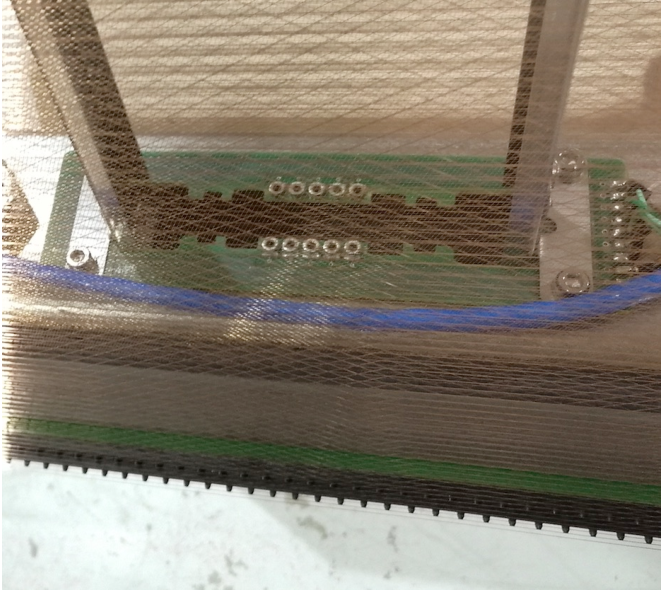
\includegraphics[height=6.cm]{pds-connector-mounted-in-apa.pdf}
	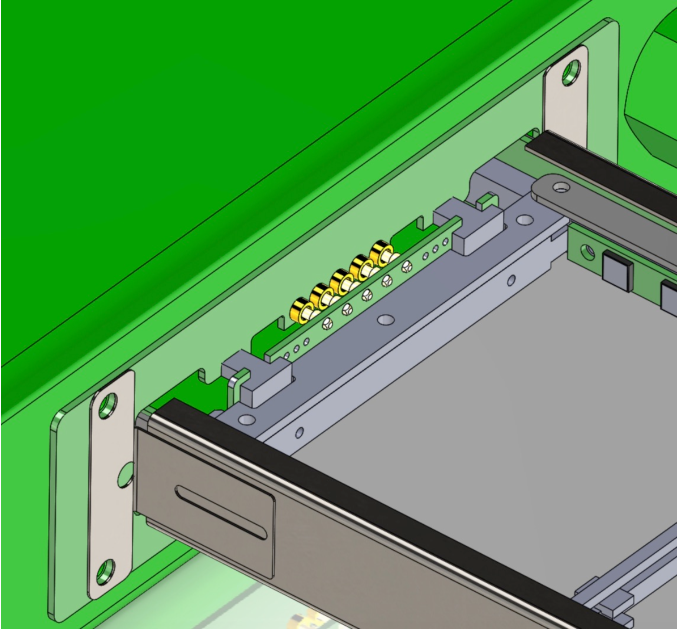
\includegraphics[height=6.cm]{pds-connector-assembly-in-apa.pdf}
\end{dunefigure}

\subsubsection{Thermal Contraction and Load Deformation}
\label{sssec:pds-thermal-load}
\textit{\bf Thermal Contraction}

During cool down from room 
to \dword{lar} temperatures,  significant relative shrinkage of module components is possible.  Mitigating these effects was a major consideration in the \dword{xarapu} module design.

Thermal expansion coefficients (CTEs) for the stainless steel \dword{apa} frames and fused-silica filter plates drove the materials selection for the \dword{xarapu} modules.  As shown in Table~\ref{tbl:fdsfpdshrink},  the relative shrinkage of FR-4 G-10 and stainless steel are well-matched and fall between the fused silica filter plates and the polystyrene WLS plates. The frame components are fabricated from FR-4 G-10, resulting in a shrinkage of the stainless steel frame structure relative to the frame of approximately \SI{1.2}{mm} along the long ($\sim$\SI{2000}{mm}) axis of the bar, minimizing the motion needed to be accounted for in the electrical connectors to the wiring harness.  The shrinkage of the frame relative to the filter plate is <~\SI{0.2}{mm}.  Both these relative shrinkage factors are accounted for in the dimensions and tolerances of the design.

The largest relative contraction of mechanical components is between the FR-4 frame and the polystyrene \dword{wls} plates. The most critical relative shrinkage is between the face of the photosensors and the \dword{wls} plate, where the \SI{92}{mm} width of the plate will shrink significantly more than the \dword{pd} module structure, resulting in more separation (approximately \SI{1.3}{mm}) between the sensor face and the plate.
%Updated comment from Franciole and Laura 6/25/19
 Simulation indicates that \dword{xarapu} performance is not strongly affected by this gap size (reducing the gap to zero, direct contact, would be beneficial but would introduce unacceptable risk of damage).  %Relative contraction along the long axis of the \dword{wls} plate, while greater in magnitude (the \SI{487.0}{mm} long plate results in a \SI{5.8}{mm} relative contraction), it is less critical to the performance of the detector and is addressed by the \dword{wls} bar mounting structure.
 The \dword{wls} plate contracts relatively more along the long axis, by \SI{5.8}{mm} for the \SI{487.0}{mm} long plate, but this affects the performance of the detector less; the \dword{wls} bar mounting structure addresses this issue.

Another important potential thermal contraction interference to track in the PD design is the relative contraction of the slots in the \dword{apa} frame and the separation of the photon detector support rails relative to the photon detector cross section.  This requirement is listed in Table~\ref{tab:specs:SP-PDS} as specification SP-PD-12, which requires that a minimum gap between the \dword{pd} module and the APA frame of \SI{0.5}{mm} be maintained after cool-down.  Specification SP-PD-08 in the same table that requires a minimum clearance of \SI{1.0}{mm} between the modules and the \dword{apa} frame at room temperature, together with the relative thermal contractions of the stainless steel \dword{apa} frame and G-10 \dword{pd} frames ensures that this specification is met.

\begin{dunetable}[Shrinkage of \dshort{pd} materials]
%{|c|c|}
{lc}
{tbl:fdsfpdshrink}
{Shrinkage of \dword{pd} module materials for a $206^{\circ}$C temperature drop}
Material 			 & Shrinkage Factor (m/m)\\ \toprowrule
Stainless Steel (304) & $2.7\times10^{-3}$\\ \colhline
FR-4 G-10 (In-plane) & $2.1\times10^{-3}$\\ \colhline
Fused Silica (Filter Plates) & $1.1\times10^{-4}$\\ \colhline
Polystyrene (WLS Bars) & $1.4\times10^{-2}$\\ 
\end{dunetable}

Mitigation of these contractions is detailed in Table~\ref{tbl:fdsfpdshrinkeffects}.

\begin{dunetable}[Relative shrinkage of \dshort{pd} components and \dshort{apa} frame]
%{|p{0.2\textwidth}|p{0.2\textwidth}|p{0.5\textwidth}l}
{p{0.2\textwidth}p{0.2\textwidth}p{0.5\textwidth}}
{tbl:fdsfpdshrinkeffects}
{Relative Shrinkage of \dword{pd} components and \dword{apa} frame, and mitigations.}
\textbf{Interface} & \textbf{Relative shrinkage} & \textbf{Mitigation} \\ \toprowrule
\dword{pd} Length to \dword{apa} width & \dword{pd} expands  \SI{1.2}{mm} relative to \dword{apa} frame & \dword{pd} affixed only at one end of \dword{apa} frame, free to expand at other end.  \SI{3}{mm} nominal clearance (beyond tolerance allowance) for expansion in design. \\ \colhline
Width of \dword{pd} in \dword{apa} Guide Rails & \dword{pd} expands \SI{.1}{mm}  relative to slot width & \dword{pd} not constrained in C-channels. C channels and tolerances designed to contain module across thermal contraction range. \\ \colhline
Width of module end mount board to stainless steel frame & Stainless frame shrinks \SI{0.1}{mm}  more than PCB & Diameter of shoulder screws and FR-4 board clearance holes selected to allow for motion. \\ \colhline
Length of WLS bar relative to FR-4 \dword{pd} frame & WLS bar shrinks \SI{5.8}{mm} relative to \dword{pd} frame & Allowed for in WLS bar mount fixtures. \\ 
\end{dunetable}

\textit{\bf \dword{pd} Mount frame deformation under static \dword{pd} load}

%\fixme{Dave: Section will remain but requires new calculations based on X-ARAPUCA design.  Will be complete by March 2019 revision. -Dave} rjw This is on Dave's todo list.

\Dword{fea} modeling of the \dword{pd} support structure was conducted to study static deflection prior to building \dword{pdsp} prototypes.  Modeling was conducted in both the vertical orientation (\dword{apa} upright, as installed in cryostat) and also horizontal orientation.  
Basic assumptions used were fully-supported fixed end conditions for the rails, 
with uniform loading of 3$\times$ \dword{pd} mass (\SI{5}{kg}) along the rails.  
Figure~\ref{fig:pds-rail} illustrates the rail deflection for the \dword{apa} in the horizontal (left) and vertical (right) orientations.
Prototype testing confirmed these calculations.  Similar modeling of final-design \dword{dune} \dword{pd} modules will be completed prior to 60\% design review.

%\fixme{Dave: are you on track to do the new modelling?}

\begin{dunefigure}[\dshort{pd} mechanical support analysis]{fig:pds-rail}
{\dword{pd} mechanical support analysis: Rail deflection for the \dword{apa} in the horizontal (left) and vertical (right) orientations.}
	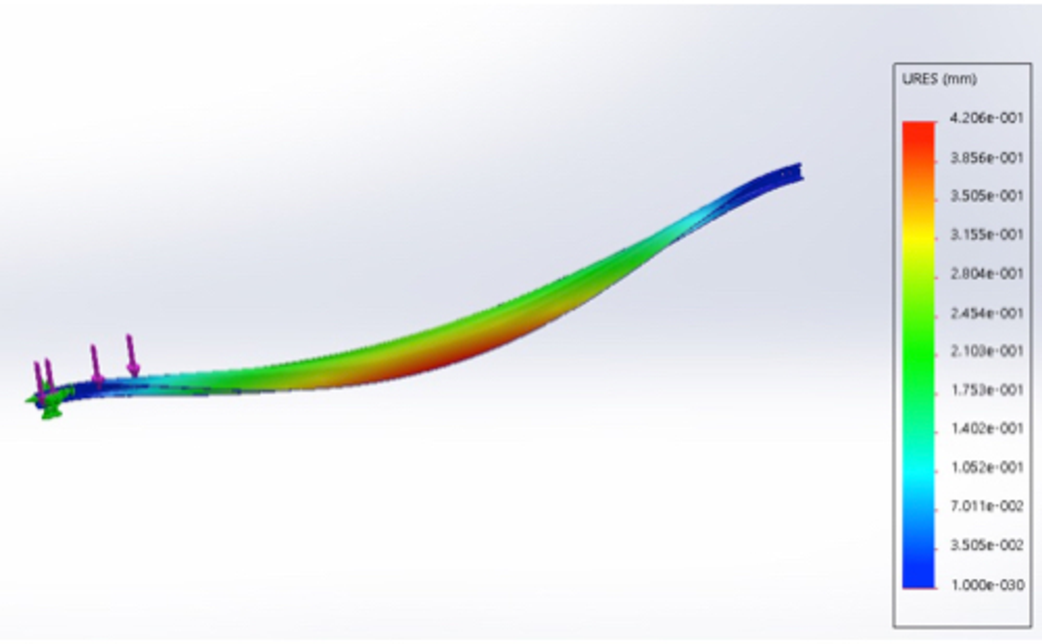
\includegraphics[height=4.5cm]{pds-rail-deflec-apa-flat.pdf} 
	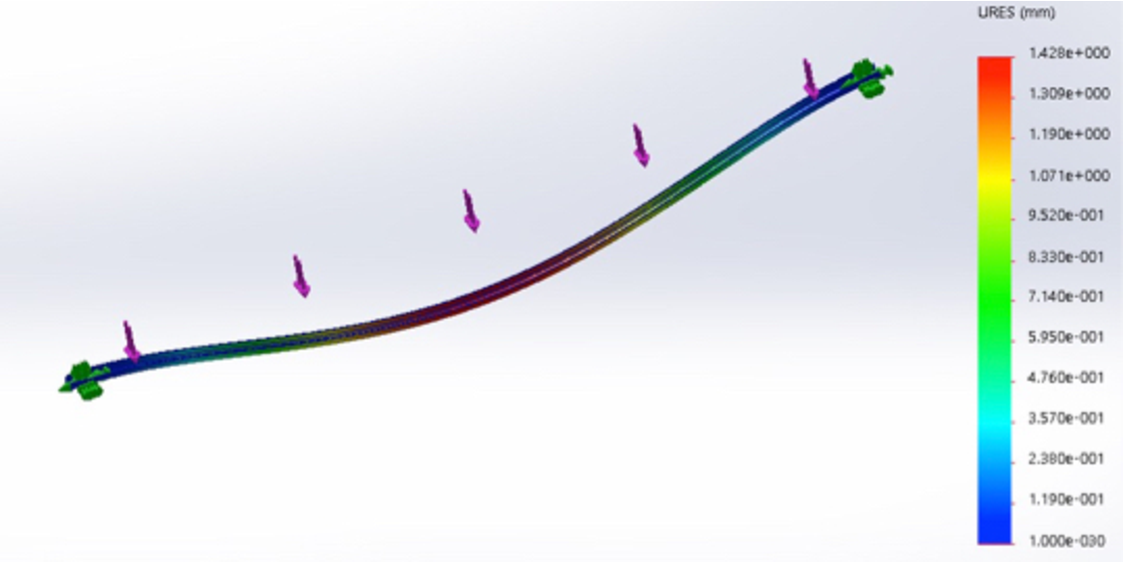
\includegraphics[height=4.5cm]{pds-rail-deflec-apa-vert.pdf}\\
\end{dunefigure}


%%%%%%%%%%%%%%%%%%%%%%%%%%%%%%%%%%
\subsection{Photosensors and Photosensor Modules}
\label{sec:fdsp-pd-assy-psm}

The use of \dwords{sipm} in noble liquids is relatively new but growing rapidly with experiments such as GERDA, MEG II, DarkSide, and nEXO which are in various stages of preparation. The collaborators of DUNE will learn from these experiments, but in principle, DUNE has a more stringent accessibility and longevity constraints. Risk mitigation through reliability engineering, process control, and vendor and collaboration testing will be a key feature of the DUNE \dword{sipm} production process.

{\textit{Reliability Engineering:}} The primary issue is the change in material properties and thermal stresses induced in the packaging due to differential coefficients of thermal expansion (CTEs). This is especially critical for interfaces, in particular
die to substrate, substrate to potting mold, potting mold to encapsulation, and solder joints to everything else. Analysis of these interfaces and collaboration with vendors to match CTEs as much as possible at these interfaces will contribute substantially to the long-term reliability of the photosensors.

{\textit{Process Control:}} Small and seemingly innocuous
changes in the photosensor fabrication process can have a big impact on the robustness of these devices at extreme temperatures. This is one of the reasons why in space applications, for instance, same-day same-batch components are utilized. Given the photosensor quantities involved, this is not feasible for the DUNE \dword{pds}, but
it will be important to establish an MoU with the vendor regarding 
strict process control once the pre-production batch has been qualified.

{\textit{Procurement:}} Potential vendors have verified that delivery of \num{100000} devices per year is a reasonable expectation so long as the purchase contract is initiated early enough.  Vendor visits to Hamamatsu and \dword{fbk} in June-July 2019 will be used as an opportunity to confirm this guidance.

{\textit{Quality Assurance:}} This will be an essential component in the photosensor risk mitigation strategy consisting of restricting the number of production batches, clearly communicating desired device and packaging parameters to the vendor, and vendor testing to
guarantee device operation down to liquid nitrogen temperatures.
Before shipment to the consortium, the vendor 
must qualify a randomly selected sample of devices from each production batch. The qualification would entail thermally stressing the devices 
with visual and electrical measurements made before and after. 

{\textit{Quality Control:}} The above strategies, while significantly lowering the risk, do not obviate the need for a strict testing regimen. Every sensor will be tested multiple times, at various stages of assembly, before installation in the \dword{spmod}.

\Dwords{sipm} are mounted in groups of six passively-ganged sensors to mounting boards, with eight mounting boards per supercell.  Passive ganging (sensors in parallel) is implemented with traces on the \dword{sipm} mounting board (\dword{pd} module), 
as was done for \dword{pdsp}.  The \dwords{sipm} are mounted using a pick-and-place machine and standard surface-mount device soldering procedures. The outputs from these mounting boards are then routed to active ganging circuits in the center of the \dword{pd} module, where they are collected into a summing amplifier and reduced to a single output channel.

The ganged analog signals exit via long cables (approximately \SI{20}{m}) for digitization outside the cryostat.
\dword{pdsp} has provided essential operational experience with a passive ganging board and signal transport provided by Teflon Ethernet Cat-6 cables, as described in Section~\ref{sec:fdsp-pd-assy-frames}.

%%%%%%%%%%%%%%%%%%%%%%%%%%%%%%%%%%
\subsection{Electronics}
\label{sec:fdsp-pd-assy-pde}

The \dword{pds} consortium gained extensive experience in manufacturing processes for electronic systems during the development of the \dword{pdsp} \dwords{ssp}.
A general description of the readout system of \dword{pdsp} can be seen in the Section~\ref{sec:fdsp-pd-pde}. Compatibility between elements designed by different institutions is guaranteed when standard procedures are followed, so the circuit design must be done in accordance with mutually agreed-upon specification documents.  A sufficient  number of units must be produced to allow %local testing and 
for testing both locally and  in the central facility; for example, in \dword{pdsp} five 12-channel  \dwords{ssp} were produced and delivered to CERN for integration testing. Twenty-four were fabricated for \dword{pdsp} operation. Similar manufacturing test programs are envisioned for \dword{dune}.

The readout electronics of the \dword{pds} will be designed and produced with similar tools and protocols as for  \dword{pdsp}. For example, %printed circuit board (
PCB layout is performed in accordance with IPC\footnote{IPC\texttrademark{}, Association Connecting Electronics Industries, \url{http://www.ipc.org/}.} specifications. Bare PCB manufacturing requirements are embedded within the Gerber file 
fabrication documents (e.g., layers, spacing, impedance, finish, testing, etc.). Components are assembled on circuit boards either by trained \dword{pd} consortium technical staff or by external assembly vendors, based on volume, and in accordance with per-design assembly specification documents. Testing occurs at %labs and universities within the 
collaboration institutions in accordance with a per-design test procedure that typically includes a mix of manual, semi-automated and automated procedures %testing 
in an engineering test bench followed by overall characterization in a system or subsystem test stand.
Other considerations and practices relevant to readout electronics production and assembly are itemized here:

\begin{itemize}

\item Components: Schematic capture is done using appropriate tools (such as OrCAD 16.6.\footnote{OrCAD\texttrademark{} schematic design tool for PCB design http://www.orcad.com} or similar toolset) available within a design facility. Design is hierarchical with common \dword{fe} page referenced multiple times, such as for all input channels. 
The schematic contains the complete bill of materials (BOM) including all mechanical parts. An electronics schematics subversion
repository or similar tool is typically used for version control and backup. Multiple internal design reviews are held before the schematic is released %to 
for layout. The BOM, stored directly within the schematic, is extracted to a spreadsheet when ordering parts. Every part specifies %is specified by 
both manufacturer and distributor information. Distributor information may be overridden by a technician at order time due to price or availability. Standard search engines such as Octopart\footnote{Octopart https://octopart.com/}, ECIA\footnote{ ECIA https://www.eciaauthorized.com} and PartMiner\footnote{PartMiner https://www.part-miner.com/} are used to check price or availability across all standard distributors. A parts-availability check %review 
is performed prior to handoff from schematic to layout since % as required 
obsolete or long lead-time parts %were 
may have been removed from the design and replaced. BOM information includes dielectric, tolerance, temperature coefficient, voltage rating, and size (footprint) to ensure that all parts are fully described.

\item Boards: Standard tools (such as the Allegro\footnote{Cadence Allegro\textregistered PCB design solution https://www.cadence.com} toolset) are available for the PCB layout. Conventional PCBs are 
controlled-impedance multilayer boards with many sets of delay-matched nets where necessary.
In usual practice, multiple previously qualified vendors bid competitively. The consortium electronics group provides the complete impedance and delay characteristics  within the layout tool, and the selected vendor cross-checks these values prior to manufacture and performs full electrical and impedance testing.  Multiple internal design reviews are held prior to release of the design.

\item Cable plant: The cabling designed will take into consideration the \dword{apa} space and will be done in close collaboration with the TPC \dword{ce} consortium to avoid crosstalk effects.  
Before making a final decision on cable procurement, we are investigating the possibility of cable manufacturing in a \dword{pds} consortium institution versus the cost of a commercial solution.  

\item Manufacturer list: In addition to the general laboratory procedures for \dword{qa}, the general practice will be to use only PCB manufacturers and external assembly vendors whose workmanship and facilities have been personally inspected by experienced production team members. All external assemblers are required to quote in accordance with an assembly specifications document describing the IPC class and specific solder chemistry requirements of the design. The BOM document will show selected and alternate suppliers where available for every component of the \dword{fe} boards.

\item \dword{fe} electronics firmware: This will be specified and updated iteratively in collaboration with other systems. The electronics working group will be responsible for responding to requests for additional firmware development, including for example, modifications to timing interface, modifications to trigger interface, and implemented sensitivity to in-spill versus not-in-spill conditions. Documents describing firmware architecture for each major change will be written and distributed to \dword{pd} and \dword{daq} working groups before implementation. An \dword{fe}  electronics users manual containing all details of new firmware will be distributed with production units when manufactured.

\item Mechanical assembly: With the mechanical assembly of electronics readout boards, it is common practice to use a \threed model generated by the layout software.   
All relevant dimensions of the PCB including connector and indicator placement is extracted as a base DXF file from which an overall exploded mechanical diagram of chassis and other mechanical parts is made.  Mechanical items such as shield plates will also be provided. It is assumed that external vendors will make the \dword{fe} chassis %will made by external vendors 
(one for the chassis, one for front and back panels) from drawings provided by the consortium.

\end{itemize}

\subsection{Calibration and Monitoring}
\label{sec:fdsp-pd-assy-CandM}

The consortium gained extensive experience in manufacturing, testing, and assembly processes 
during the development of the calibration and monitoring system for \dword{pdsp}.
A general description of the proposed calibration and monitoring system can be seen in  Section~\ref{sec:fdsp-pd-CandM}. 

The design and production of the calibration modules including electronics circuitry,  \dword{fpga} implementation for light-source controls, optical timing/trigger and \dword{daq} communication protocols, and UV light sources, closely follows the process described in Section~\ref{sec:fdsp-pd-assy-pde}.

Design and selection of cold diffuser components and selection of cold and warm quartz fiber components follows requirements derived from interface considerations with \dword{hv},  \dword{cpa} and cryostat systems,  
and was tested in \dword{pdsp}.
Installation, \dword{qa} and \dword{qc} of optical fibers is performed during the \dword{cpa} installation process, with diffusers and \dword{cpa} fibers pre-installed on the \dword{cpa}s.

Installation of fibers that connect \dword{cpa}s %'s fiber connections 
to the optical feedthrough penetrations at the cryostat will be defined with the \dword{dss} and cryostat teams, based on installation experience in \dword{pdsp}. 

\subsection{Outline of PD System Assembly Plan}
\label{sec:fdsp-pd-assy-Assby-plan}

The Photon Detector Consortium is composed of many institutions in North and South America and Europe; fabrication of the system will occur at many locations throughout the consortium.  Here we present an outline of our production plan.  The schedule interfaces implicit in this assembly program will be detailed in the overall project schedule.

\begin{itemize}

\item Photosensors, mounting and active ganging:  %Photosensor procurement, testing, and the active ganging circuit assembly will be performed by 
Italian groups funded by INFN (and their associated universities) will procure, test, and assemble the active ganging circuits for the \dword{pds}. Photosensor mounting board assembly will likely be outsourced to a yet to be selected external firm.%, which has yet to be selected.

The groups that are most involved in the \dword{pds} are Bologna, Genova, Milano, Milano-Bicocca, and Laboratori Nazionali del Sud.  Other Italian groups have also expressed interest in joining.  We will allocate tasks among the interested groups prior to the final design review.

Following assembly, these components and their associated \dword{qc} documentation will be shipped to \dword{unicamp} for assembly into \dword{pd} modules.

\item Light collector modules:  Light collector modules will be fabricated primarily in Brazil.  

Dichroic filters and wavelength shifting plates will be procured and received by a combination of CTI Campinas and the National Laboratory of Synchrotron Light (also in Campinas), where they will undergo reception \dword{qc} testing.

Following testing, the dichroic filters will be delivered to \dword{unicamp} for coating with \dword{ptp} in their in-house vacuum deposition system.

The module mechanical components are also the responsibility of \dword{unicamp}.  This includes the FR-4 G-10 components (which will be fabricated in-house at \dword{unicamp}), signal routing circuit boards, module electrical connectors, and other miscellaneous components (purchased externally) required to fabricate the modules.

Module assembly and initial \dword{qc} testing will happen at \dword{unicamp}.

Following assembly, the tested modules and all the associated \dword{qc} documentation will be shipped to a reception center in the US, where they will be retested and stored in the \dword{sdwf} until required for integration into the APAs underground.

%\fixme{Rails moved into US Scope dww 10/11/19}

\item \dword{apa} support rails and electrical connectors:  Stainless steel rails and associated hardware for supporting the PD modules inside the \dword{apa} will be fabricated by vendor in the \dword{us}.  Components for cable connection between the upper and lower APAs, and cable management pieces, will be procured from vendors, assembled, and tested in the \dword{us}.  

Following assembly and testing, these components will be shipped to \dword{apa} frame assembly sites for integration into the frames prior to wire wrapping.

\item Readout electronics and \dword{daq} interface:  The front end electronics and \dword{daq} interfaces will be built by a collaboration of Latin American countries, particularly Colombia, Peru, and Paraguay, with engineering support from \dword{fnal} and the University of Michigan in the US. 

The front end electronics, communications boards, and external cabling between them and the \dword{daq} will be designed by collaboration engineers, fabricated, or purchased from external vendors, and tested at collaboration institutions.  While the exact distribution of effort is still being settled, interested institutions in Colombia include Antonio Narino University (UAN) and the Escuela de Ingenieria de Antioquia (EIA).  In Peru, they include the Universidad Nacional de Ingenieria de Peru.

\dword{daq}/\dword{pd} interface firmware development will be conducted by Paraguay, particularly the Universidad National de Asuncion (FIUNA), in conjunction with UAN in Colombia.

Following assembly and testing, components will be shipped to a reception center in the US for inspection then stored at the \dword{sdwf} until needed.

%\fixme{Cables divided to US and international scope dww 10/11/19}
\item Cables:  Materials for cables and connectors inside the \dword{apa} frames will be purchased, assembled and tested in the \dword{us}.  Cables between the APA and the cryostat flange, as well as those between the flange and the \dword{daphne} electronics, will be purchased by \dword{unicamp} and assembled and tested at their facilities.
Following testing, the cables and their associated \dword{qc} documentation will be assembled into groups of 20 cable sets (one \dword{apa} stack) and shipped to the \dword{sdwf} for storage until needed for installation.  Cables intended to be routed inside the \dword{apa} frames will be shipped directly to the \dword{apa} frame assembly facilities.

\item Monitoring system: The monitoring system including \dword{led} drivers, optical fibers, and diffusers will be designed, fabricated and tested in the US by the South Dakota School of Mines and Technology and Argonne National Laboratory. 

Following assembly and testing, the system will be stored at the \dword{sdwf} until needed for installation.

\end{itemize}

